%% =====================================================================
%% MDPI Micromachines research article — manuscript body
%%
%% HOW TO COMPILE
%% -------------------------------------------------------------------
%% This file is the manuscript BODY. It is meant to be dropped into the
%% official MDPI "Micromachines" Overleaf template, which supplies the
%% class file Definitions/mdpi.cls, the style mdpi.bst, the MDPI logo,
%% and the rest of the Definitions/ tree. Steps:
%%   1. Open the MDPI Micromachines LaTeX template on Overleaf
%%      (Menu > New Project > Templates > MDPI Micromachines), or download
%%      the LaTeX package from https://www.mdpi.com/authors/latex .
%%   2. Replace the template's main .tex body with the contents of THIS
%%      file, keeping the template's Definitions/ folder, the bibliography
%%      file references.bib, and the figures/ folder alongside it.
%%   3. Compile with pdfLaTeX -> BibTeX -> pdfLaTeX -> pdfLaTeX.
%%
%% RECLASSIFICATION NOTE
%% -------------------------------------------------------------------
%% To retarget this manuscript to the MDPI journal "Biosensors" instead
%% of "Micromachines", change the journal token in \documentclass below
%% from "micromachines" to "biosensors" (single-word edit); the rest of
%% the file is journal-agnostic.
%% =====================================================================

\documentclass[micromachines,article,submit,pdftex,moreauthors]{Definitions/mdpi}

% --- Optional packages used in the body (most are loaded by mdpi.cls) ---
\usepackage{booktabs}

% --- Running-head / journal metadata (kept light; template fills the rest) ---
\firstpage{1}
\makeatletter
\setcounter{page}{\@firstpage}
\makeatother
\pubvolume{1}
\issuenum{1}
\articlenumber{0}
\pubyear{2026}
\copyrightyear{2026}
\datereceived{}
\daterevised{}
\dateaccepted{}
\datepublished{}
\hreflink{https://doi.org/}

% =====================================================================
% FRONT MATTER
% =====================================================================

\Title{$\mu$Flow: A Modeling Platform for Microfluidic Hall-Effect
Magnetic Bead Detection with Parametric Design Optimization}

% Short title used in running head and the suggested citation line
\TitleCitation{$\mu$Flow: A Modeling Platform for Microfluidic Hall-Effect
Magnetic Bead Detection}

\newcommand{\orcidauthorA}{0000-0000-0000-0000}
\newcommand{\orcidauthorB}{0000-0000-0000-0000}

\Author{Harshitha Govindaraju $^{1,}$*\orcidA{} and Umer Hassan $^{1}$\orcidB{}}

% Authors for metadata / running head
\AuthorNames{Harshitha Govindaraju and Umer Hassan}

% Citation form of author list
\AuthorCitation{Govindaraju, H.; Hassan, U.}

\address{%
$^{1}$ \quad Department of Electrical and Computer Engineering, Rutgers,
The State University of New Jersey, 94 Brett Road, Piscataway, NJ 08854, USA;
umer.hassan@rutgers.edu}

\corres{Correspondence: harshitha.govindaraju@rutgers.edu}

% =====================================================================
% ABSTRACT (canonical text from the reframe brief)
% =====================================================================
\abstract{Microfluidic Hall-effect biosensors detect superparamagnetic bead
labels as they flow past a thin-film Hall element in a microchannel. Designing
such a device couples bead magnetization, stray-field distribution, Hall
transport, and channel flow across a dozen geometric, material, and operational
parameters, a space that finite-element solvers explore only at minutes to hours
per configuration. We present a coupled closed-form analytical model of this
signal chain: Clausius--Mossotti bead magnetization with a volume-fraction
correction, a point-dipole stray field, a volume-averaged Hall voltage with
geometric correction, Poiseuille transport, and a Johnson--Nyquist/Hooge $1/f$
noise framework, evaluated across a database of 12 sensor platforms spanning
graphene, III--V semiconductors, Si CMOS, bismuth, and topological insulators.
Benchmarked against a companion COMSOL FEM-BEM study, the model reproduces the
Hall voltage to within 4.8\% at a favorable bead-to-sensor area ratio; at
off-optimum geometries the point-dipole approximation deviates by 22\% and 16\%,
consistent with its known near-field limit at $h/r_b = 1$. The model yields design
rules, including a bead-to-sensor area-ratio optimum of 0.1--0.5 that matches the
independent noise-optimal width criterion of Mihajlovi\'{c} et al.\ and a
cross-material signal-to-noise ranking, and it is consistent with the
order-of-magnitude signal levels reported in published InAs and Si CMOS detection
experiments. We provide the model as an open, no-install browser implementation
with an in-app 2D axisymmetric magnetostatic FEM solver that quantifies where the
dipole approximation degrades.}

\keyword{microfluidics; Hall effect; magnetic bead detection; biosensor;
analytical model; design optimization}

\begin{document}

% =====================================================================
\section{Introduction}
\label{sec:intro}
% =====================================================================

Microfluidic Hall-effect sensors detect individual superparamagnetic beads by
measuring the transient stray magnetic field as labeled analytes flow past a
thin-film Hall element embedded in a microchannel floor. The approach has been
demonstrated across multiple sensor platforms. Ejsing et al.\ measured
\SI{0.3}{\micro\volt} signals from \SI{2}{\micro\meter} beads with a planar Hall
sensor \cite{ejsing2004}. Mihajlovi\'{c} et al.\ detected a single commercial
\SI{1.2}{\micro\meter} bead with an InAs quantum-well micro-Hall sensor, reporting
a \SI{105}{\nano\volt} noise floor and a minimum detectable stray-field change of
${\sim}\SI{4.3}{\micro\tesla}$ at a \SI{40}{\micro\ampere} bias \cite{mihajlovic2005}.
Shah et al.\ integrated CVD graphene Hall sensors
($S_I = \SI{175}{\volt\per\ampere\per\tesla}$) into a PDMS microchannel and
detected ferrofluid-loaded model beads flowing in protein buffer and diluted
blood, with sensor stability validated in whole blood \cite{shah2023}. Gabureac et al.\ resolved single
\SI{1}{\micro\meter} beads with a \SI{500}{\nano\meter} nanocomposite Hall sensor
and reported \SIrange{100}{500}{\nano\volt} signals \cite{gabureac2013}. The
diversity of viable platforms, which now spans graphene
\cite{dauber2015,kaidarova2021}, III--V semiconductors
\cite{mihajlovic2005,gilbertson2011}, Si CMOS \cite{besse2002}, and topological
insulators \cite{saeed2024}, makes material selection nontrivial because the
detected signal depends on the coupled interaction of several physics domains.

The design challenge arises from several interacting effects. The magnetization of
the bead in the applied field depends on its ferrite content and effective
susceptibility through the Clausius--Mossotti relation. The spatial distribution
of the bead's dipolar stray field decays as $1/r^3$ and changes sign at lateral
offsets. The Hall voltage is produced by averaging this inhomogeneous field over
the sensor active volume, so the signal depends jointly on bead size and sensor
footprint. The hydrodynamic transport determines the bead trajectory and transit
time through the sensing zone via the Poiseuille velocity profile. Commercial
finite-element tools such as COMSOL Multiphysics can model each of these domains,
but setting up a coupled magnetostatic-hydrodynamic simulation requires a software
license and minutes to hours of computation per configuration. Our companion study
used a COMSOL FEM-BEM model to compare three sensor geometries and four
semiconductor platforms, requiring more than 200 individual simulations
\cite{govindaraju2025}. Jebari et al.\ reported that their 3D multiphysics
simulation of a microfluidic immunosensor required coupled Navier--Stokes,
convection-diffusion, and magnetostatic solvers across multiple geometry variants,
each taking tens of minutes per configuration \cite{jebari2024}. Closed-form
analytical work covers the individual modules in isolation: point-dipole stray
fields \cite{griffiths}, planar Hall voltage \cite{popovic2004}, and
Poiseuille flow \cite{hewlin2023}. The noise-optimal sensor geometry, in which
the sensor active area is comparable to the bead footprint, identified by
Mihajlovi\'{c} et al.\ from $1/f$-limited noise analysis of InAs micro-Hall
sensors \cite{mihajlovic2007}, addresses geometry but not the full signal chain. No open model couples these modules into a single,
parameterized signal chain that a non-specialist can evaluate without a commercial
solver.

This paper presents such a model and the design rules that follow from it. The
contributions, in order of priority, are: (i)~a coupled closed-form analytical
model of the complete microfluidic Hall-effect bead-detection signal chain,
validated against a FEM-BEM benchmark to within a few percent in its regime of
validity; (ii)~design rules extracted from the model, including a bead-to-sensor
area-ratio optimum of 0.1--0.5 that coincides with the independent noise-optimal
width criterion of Mihajlovi\'{c} et al.\ \cite{mihajlovic2007}, a cross-material
signal-to-noise ranking, and a flow-velocity detection window; and (iii)~an open,
no-install browser implementation, with an in-app 2D axisymmetric magnetostatic
FEM solver, that serves as the reproducibility artifact and quantifies where the
point-dipole approximation degrades. The implementation is deployed at
\url{https://uflow.studio} and its source is released under AGPL-3.0-or-later.

% =====================================================================
\section{Model and Methods}
\label{sec:model}
% =====================================================================

The model implements the analytical signal chain validated in our companion
COMSOL FEM-BEM study \cite{govindaraju2025}. We describe each component, the noise
framework, the microfluidic transport, the material database, and the open browser
implementation that evaluates the model and provides an independent FEM check.

% ---------------------------------------------------------------------
\subsection{Bead Magnetization}
\label{sec:magnetization}

Each superparamagnetic bead of radius $r_b$ contains magnetic nanoparticle (NP)
cores with core relative permeability $\mu_r$ dispersed in a polymer matrix at
magnetic volume fraction $\phi$. The induced magnetic dipole moment is
\begin{equation}
m = \frac{4}{3}\pi r_b^3 \, \phi \, \chi_{\text{eff}} \, \frac{B_0}{\mu_0},
\label{eq:moment}
\end{equation}
where $\mu_0 = 4\pi \times 10^{-7}$~\si{\tesla\meter\per\ampere} is the vacuum
permeability, $\phi$ is the volume fraction of the magnetic phase
(Table~\ref{tab:beads}), and $\chi_{\text{eff}}$ is the Clausius--Mossotti effective
susceptibility of the core ferrite material:
\begin{equation}
\chi_{\text{eff}} = \frac{3(\mu_r - 1)}{\mu_r + 2}.
\label{eq:clausius}
\end{equation}
For magnetite ($\mu_r = 10$), Equation~\eqref{eq:clausius} gives
$\chi_{\text{eff}} = 2.25$. The factor $\phi$ in Equation~\eqref{eq:moment} is
needed for composite beads: Dynabeads M-280 contain ${\sim}5\%$ iron oxide by
volume (computed from the \SI{118}{mg/g} iron content reported by Fonnum et al.\
\cite{fonnum2005}), so their effective moment is ${\sim}20\times$ smaller than a
solid magnetite sphere of the same diameter. For the COMSOL validation beads,
$\phi = 1$ (pure magnetite).

This linear magnetization model is valid in the sub-saturation regime
($B_0 \lesssim \SI{200}{\milli\tesla}$ for magnetite NPs with
$d_\text{NP} \approx \SI{16}{\nano\meter}$). At higher fields the NP moments
approach saturation and a Langevin ensemble model is required
\cite{elfimova2019,henrard2019}; the implementation displays a warning when
$B_0$ exceeds \SI{200}{\milli\tesla} with commercial bead presets. For practical
microfluidic assays operating at $B_0 = \SIrange{20}{100}{\milli\tesla}$, the
linear Clausius--Mossotti model is appropriate \cite{ota2019}.

% ---------------------------------------------------------------------
\subsection{Point-Dipole Stray Field}
\label{sec:strayfield}

The axial component of the magnetic field from the induced point dipole, displaced
by $(\Delta x, \Delta y, \Delta z)$ from a field point, is \cite{griffiths}
\begin{equation}
B_z(\Delta x, \Delta y, \Delta z) = \frac{\mu_0}{4\pi} \, m \,
\frac{2\Delta z^2 - \Delta x^2 - \Delta y^2}
{\left(\Delta x^2 + \Delta y^2 + \Delta z^2\right)^{5/2}}.
\label{eq:dipole}
\end{equation}
The point-dipole form is the leading term of a multipole expansion and loses
accuracy when the bead-sensor separation approaches the bead radius
($h/r_b \sim 1$) \cite{griffiths}; the built-in FEM solver
(Section~\ref{sec:fem}) quantifies this deviation for each geometry, agreeing
with the dipole model to within a few percent at $h/r_b > 3$ and diverging as
$h/r_b \to 1$. The FEM solver provides a direct comparison between this
approximation and a full volumetric magnetostatic solution, so the dipole-model
validity can be checked for any bead-sensor configuration.

Equation~\eqref{eq:dipole} produces a characteristic spatial signature: $B_z$ is
positive directly above and below the dipole, crosses zero at
$\Delta z^2 = (\Delta x^2 + \Delta y^2)/2$, and becomes negative at large lateral
offsets. As a bead traverses the sensor along the channel axis, the volume-averaged
field traces a bipolar pulse whose amplitude and width depend on the bead-sensor
distance and the sensor footprint.

% ---------------------------------------------------------------------
\subsection{Volume-Averaged Hall Voltage}
\label{sec:hallvoltage}

The Hall voltage depends on the average $B_z$ over the sensor volume, not on the
surface field at a single point. The model computes this by midpoint quadrature
over an $n_{xy} \times n_{xy} \times n_z$ grid spanning the sensor volume (width
$w$, length $l$, thickness $t$):
\begin{equation}
\langle B_z \rangle = \frac{1}{n_{xy}^2 \, n_z}
\sum_{i=1}^{n_{xy}} \sum_{j=1}^{n_{xy}} \sum_{k=1}^{n_z}
B_z(\Delta x_i, \Delta y_j, \Delta z_k),
\label{eq:avgbz}
\end{equation}
where each grid point samples Equation~\eqref{eq:dipole}. The resulting Hall
voltage change is
\begin{equation}
\Delta V_H = G \, R_H \, \sigma \, \langle B_z \rangle \, V_{\text{bias}},
\label{eq:vh}
\end{equation}
where $R_H$ is the Hall coefficient (\si{\meter\cubed\per\coulomb}), $\sigma$ is the
sensor conductivity (\si{\siemens\per\meter}), $V_{\text{bias}}$ is the applied bias
voltage, and $G \in [0.5, 1.0]$ is a geometric correction factor that accounts for
current spreading in non-square Hall crosses \cite{popovic2004}. For a symmetric
Greek-cross geometry, $G \approx 1$; for long, narrow Hall bars ($l/w > 3$), $G$
approaches the ideal value of 1; for short, wide geometries ($l/w < 1$), $G$ can
drop below 0.7 \cite{popovic2004}. The default is $G = 1$ (square geometry), with
user adjustment available. For the three benchmark designs in
Reference~\cite{govindaraju2025}, $R_H = \SI{1.25e-3}{\meter\cubed\per\coulomb}$,
$\sigma = \SI{1040}{\siemens\per\meter}$, and $G = 1$.

For the 12 material presets (Section~\ref{sec:materials}), the Hall coefficient is
computed from the carrier density. For two-dimensional materials with sheet carrier
density $n_s$ (\si{\per\meter\squared}),
\begin{equation}
R_H^{\text{2D}} = \frac{1}{n_s \, e}, \qquad S_I = \frac{1}{n_s \, e},
\label{eq:rh2d}
\end{equation}
where $e = \SI{1.6e-19}{\coulomb}$ and $S_I$ is the current-related sensitivity
(\si{\volt\per\ampere\per\tesla}). For three-dimensional materials with bulk carrier
density $n$ (\si{\per\meter\cubed}) and film thickness $t$,
\begin{equation}
R_H^{\text{3D}} = \frac{1}{n \, e}, \qquad
S_I = \frac{R_H^{\text{3D}}}{t} = \frac{1}{n \, e \, t}.
\label{eq:rh3d}
\end{equation}
For gate-tunable 2D materials (graphene variants, Bi$_2$Se$_3$), the carrier density
varies with the applied gate voltage $V_g$ relative to the charge neutrality point
$V_{\text{CNP}}$:
\begin{equation}
n_s(V_g) = n_{s,0} + \frac{C_{\text{ox}}}{e}\,|V_g - V_{\text{CNP}}|,
\label{eq:gate}
\end{equation}
where $n_{s,0}$ is the residual carrier density at neutrality and $C_{\text{ox}}$ is
the gate oxide capacitance per unit area. Reducing $n_s$ increases the Hall
coefficient but also increases the device resistance and associated Johnson noise,
so the gate slider exposes the sensitivity-noise trade-off directly.

Tu et al.\ showed that the detected signal from a planar Hall sensor scales linearly
with the sensor active area when the bead is centered but drops sharply when the
bead is offset laterally \cite{tu2009}; the volume averaging in
Equation~\eqref{eq:avgbz} captures this spatial dependence. Uddin et al.\
demonstrated through FEM optimization that elliptical sensor geometries can increase
the effective sensing area by \SIrange{15}{20}{\percent} compared with square
designs of the same footprint \cite{uddin2022}.

% ---------------------------------------------------------------------
\subsection{Noise and Detection Limits}
\label{sec:noise}

Whether a bead is detectable depends not only on the Hall voltage magnitude but on
the signal-to-noise ratio. The model implements a noise framework covering the
dominant noise sources in Hall sensors: Johnson--Nyquist (thermal) noise and Hooge
$1/f$ (flicker) noise. The sheet resistance of the sensor is
\begin{equation}
R_\square = \frac{1}{n_\text{tot} \, e \, \mu},
\label{eq:rsq}
\end{equation}
where $n_\text{tot}$ is the total carrier density and $\mu$ is the carrier mobility.
For a square sensor biased at $V_\text{bias} = I_\text{bias} R_\square$, the thermal
noise voltage in a measurement bandwidth $\Delta f$ is
\begin{equation}
V_\text{th} = \sqrt{4 k_B T R_\square \Delta f},
\label{eq:thermal}
\end{equation}
where $k_B$ is the Boltzmann constant and $T$ is the temperature. The $1/f$ noise
voltage, following the Hooge model \cite{xu2013,huang2014}, is
\begin{equation}
V_{1/f} = V_\text{bias}\sqrt{\frac{\alpha_H}{N}\,
\ln\!\left(1 + \frac{\Delta f}{f_\text{op}}\right)},
\label{eq:flicker}
\end{equation}
where $\alpha_H$ is the dimensionless Hooge parameter,
$N = n_\text{tot} A$ is the total carrier count in the sensor active area $A$, and
$f_\text{op}$ is the operating frequency. The total noise voltage and detection
metrics are
\begin{equation}
V_n = \sqrt{V_\text{th}^2 + V_{1/f}^2}, \quad
\text{SNR} = \frac{|\Delta V_H|}{V_n}, \quad
B_\text{min} = \frac{V_n}{|S_I| \, I_\text{bias}},
\label{eq:snr}
\end{equation}
where $B_\text{min}$ is the minimum detectable field per unit bandwidth. A bead is
considered detectable when $\text{SNR} > 3$.

The Hooge parameter $\alpha_H$ varies by several orders of magnitude across sensor
platforms, from ${\sim}10^{-5}$ for high-quality encapsulated graphene to
${\sim}10^{-2}$ for disordered thin films \cite{xu2013,huang2014}. This
material-dependent noise floor shapes the cross-material comparison: a platform with
high mobility and high $\alpha_H$ may produce a weaker SNR than a lower-mobility
platform with superior noise performance, a trade-off that $\Delta V_H$ alone cannot
capture. The model accepts a user-specified $\alpha_H$ and computes the noise floor,
SNR, and $B_\text{min}$ alongside $\Delta V_H$ for every configuration, enabling
noise-aware design optimization when published noise characterization data are
available for the platform of interest.

% ---------------------------------------------------------------------
\subsection{Microfluidic Transport}
\label{sec:transport}

Bead trajectories follow Poiseuille flow in a rectangular microchannel. For a
channel with height $H$ and width $W \gg H$ (aspect ratio ${>}10{:}1$, so that
sidewall drag is negligible), the streamwise velocity at vertical position $y$ is
\begin{equation}
v(y) = \frac{3}{2}\,\bar{v}\left[1 - \left(\frac{2y}{H} - 1\right)^2\right],
\label{eq:poiseuille}
\end{equation}
where $\bar{v}$ is the mean flow velocity. Beads at the channel center ($y = H/2$)
travel at $1.5\bar{v}$, while those near the walls approach zero velocity. Hewlin
and Edwards used this parabolic profile to model particle trajectories in a Y-shaped
microfluidic channel, confirming that laminar-flow assumptions hold for Reynolds
numbers below ${\sim}1$ in channels of comparable dimensions \cite{hewlin2023}.
Khashan et al.\ showed that coupling Poiseuille flow with magnetophoretic body
forces enables selective sorting of labeled versus unlabeled particles in similar
geometries \cite{khashan2024}.

The model distinguishes two height parameters: $h$, the bead-center distance above
the sensor surface, and $H$, the channel height. Only $h$ enters the dipole
stray-field formula and therefore directly drives $\Delta V_H \propto 1/h^3$; $H$
does not appear in the signal formula but bounds where $h$ can sit (geometric
constraint $r_b \le h \le H - r_b$) and shapes the velocity profile via the $y/H$
dependence. In fixed-height mode all beads share the same $h$, which isolates the
influence of sensor, bead, or material parameters. In range mode each bead's $h$ is
drawn from a uniform distribution over the allowed interval, so the per-bead signals
span the $1/h^3$ decay. An optional magnetophoretic drift component pulls beads
toward the sensor surface at a rate proportional to the local field gradient,
modeling magnetic capture. The uniform sampling is a deliberate worst-case baseline:
in a flowing channel the equilibrium height distribution is biased toward the floor
by sedimentation (Stokes velocity
$v_s = \tfrac{2}{9}\Delta\rho g r_b^2/\eta \approx \SI{2}{\micro\meter\per\second}$
for a \SI{2.8}{\micro\meter} M-280 Dynabead in water) over channel residence times,
which concentrates beads where $1/h^3$ signals are strongest, so detected SNR in
practice tends to exceed the uniform-range prediction. The bead position is updated
each frame as $x(t + \Delta t) = x(t) + v(y)\Delta t$, with adaptive sub-stepping
that caps the displacement per sub-step at $0.4\,w_\text{sensor}$ so that the narrow
signal peak is not stepped over between frames.

% ---------------------------------------------------------------------
\subsection{Material Database}
\label{sec:materials}

The model carries 12 Hall sensor material presets spanning graphene, III--V
semiconductors, Si CMOS, bismuth, and topological-insulator families
(Table~\ref{tab:materials}). Each preset specifies the carrier mobility $\mu$, the
carrier density ($n_s$ for 2D or $n$ for 3D), and the dimensionality. All parameter
values were extracted from peer-reviewed publications as indicated. For gate-tunable
2D materials (graphene variants, Bi$_2$Se$_3$), a gate voltage can be applied via
Equation~\eqref{eq:gate} to shift the operating point along the sensitivity-noise
trade-off curve. Since $\Delta V_H \propto \mu S_I \langle B_z\rangle V_{\text{bias}}$
and $S_I \propto 1/n_s$, the Hall voltage is proportional to the mobility for a given
geometry; the database therefore supports cross-platform comparison under identical
bead-channel conditions.

\begin{table}[H]
\caption{Material property database. $\mu$: carrier mobility;
$S_I = 1/(n_s e)$ for 2D materials; $R_H = 1/(ne)$ for 3D. All values at room
temperature.\label{tab:materials}}
\newcolumntype{C}{>{\centering\arraybackslash}m{3.0cm}}
\begin{tabularx}{\textwidth}{lrrX}
\toprule
\textbf{Material} & \boldmath$\mu$ \textbf{(cm$^2$/Vs)} &
\textbf{\boldmath$S_I$ or $R_H$} & \textbf{Refs.} \\
\midrule
\multicolumn{4}{@{}l}{\textit{Graphene (2D, gate-tunable)}} \\
CVD graphene  & 3000   & 1250\,V/AT & \cite{xu2013,huang2014} \\
Graphene/hBN  & 40{,}000 & 5700\,V/AT & \cite{dauber2015,ouaj2025} \\
Graphene/SiC  & 3000   & 83\,V/AT   & \cite{ciuk2019,panchal2012} \\
\midrule
\multicolumn{4}{@{}l}{\textit{III--V semiconductors (2D)}} \\
GaAs/AlGaAs   & 7000   & 1250\,V/AT & \cite{haned2003,kunets2008,boero2003} \\
AlGaN/GaN     & 1500   & 62.5\,V/AT & \cite{zhang2021,koide2012} \\
InAs/AlSb     & 22{,}000 & 625\,V/AT  & \cite{mihajlovic2005,boero2003,heremans1993} \\
InSb QW       & 42{,}000 & 1250\,V/AT & \cite{gilbertson2011,kunets2009,sandhu2004} \\
\midrule
\multicolumn{4}{@{}l}{\textit{III--V semiconductors (3D)}} \\
InSb MBE      & 35{,}000 & $3.1{\times}10^{-4}$\,m$^3$/C & \cite{togawa2005,okamoto2003,sandhu2004,kazakova2009} \\
InAs film     & 22{,}000 & $4.2{\times}10^{-5}$\,m$^3$/C & \cite{boero2003,heremans1993,mihajlovic2005} \\
\midrule
\multicolumn{4}{@{}l}{\textit{Other platforms}} \\
Si CMOS       & 1400   & $6.3{\times}10^{-4}$\,m$^3$/C & \cite{besse2002,boero2003} \\
Bismuth       & 15{,}000 & $2.1{\times}10^{-5}$\,m$^3$/C & \cite{komnik1975,heremans1993} \\
Bi$_2$Se$_3$ TI & 3000 & 312\,V/AT & \cite{saeed2024,koirala2015} \\
\bottomrule
\end{tabularx}
\end{table}

Table~\ref{tab:beads} lists the bead presets. The first three correspond to
commercially available superparamagnetic beads widely used in immunoassay and
cell sorting; the last three match the magnetite beads used in the COMSOL
validation study \cite{govindaraju2025}.

\begin{table}[H]
\caption{Bead library. $\phi$: magnetic (iron oxide) volume fraction, computed from
the iron content (mg/g) reported by Fonnum et al.\ \cite{fonnum2005} using
$\rho_{\gamma\text{-Fe}_2\text{O}_3} = \SI{4.9}{g/cm^3}$. $\mu_r$: relative
permeability of the ferrite core.\label{tab:beads}}
\begin{tabularx}{\textwidth}{lCCCX}
\toprule
\textbf{Bead Preset} & \boldmath$d_b$ \textbf{($\mu$m)} &
\boldmath$\phi$ \textbf{(\%)} & \boldmath$\mu_r$ & \textbf{Source} \\
\midrule
Dynabeads MyOne   & 1.05 & 13$^{a}$ & 10 & \cite{fonnum2005} \\
Dynabeads M-280   & 2.83 & 5$^{a}$  & 10 & \cite{fonnum2005} \\
Dynabeads M-450   & 4.50 & 9$^{a}$  & 10 & \cite{fonnum2005} \\
Magnetite 2\,$\mu$m  & 2.00 & 100 & 10 & \cite{govindaraju2025} \\
Magnetite 6\,$\mu$m  & 6.00 & 100 & 10 & \cite{govindaraju2025} \\
Magnetite 10\,$\mu$m & 10.0 & 100 & 10 & \cite{govindaraju2025} \\
\bottomrule
\end{tabularx}
\noindent\footnotesize{$^{a}$ Volume fraction computed from Fonnum et al.'s iron
content: MyOne \SI{255}{mg/g}, M-280 \SI{118}{mg/g}, M-450 \SI{202}{mg/g};
converted via Fe$_2$O$_3$ stoichiometry and bead density.}
\end{table}

% ---------------------------------------------------------------------
\subsection{Open Browser Implementation}
\label{sec:implementation}

The model is provided as an open implementation that evaluates
Equations~\eqref{eq:moment}--\eqref{eq:snr} in a web browser. The application is a
single HTML file (${\sim}\num{3000}$ lines) that loads React~18 (UMD build) for
reactive state management and Three.js r160 (ES module) for the WebGL 3D scene from
CDN URLs; an HTML5 Canvas renders the 2D signal trace, the parametric sweep charts,
and the FEM field visualization. The architecture requires no build tools, package
managers, or server-side dependencies, and the same file can be opened from a local
filesystem. A pure-JavaScript physics engine exposes the bead-moment,
point-dipole, volume-average, and flow-velocity functions plus a helper that derives
the Hall coefficient, conductivity, and sensitivity from material parameters and an
optional gate voltage. Figure~\ref{fig:architecture} shows the data-flow
architecture: user interactions update React state, which triggers the memoized
physics computations, whose results feed the Three.js scene, the Canvas trace, and
the FEM solver.

\begin{figure}[H]
\centering
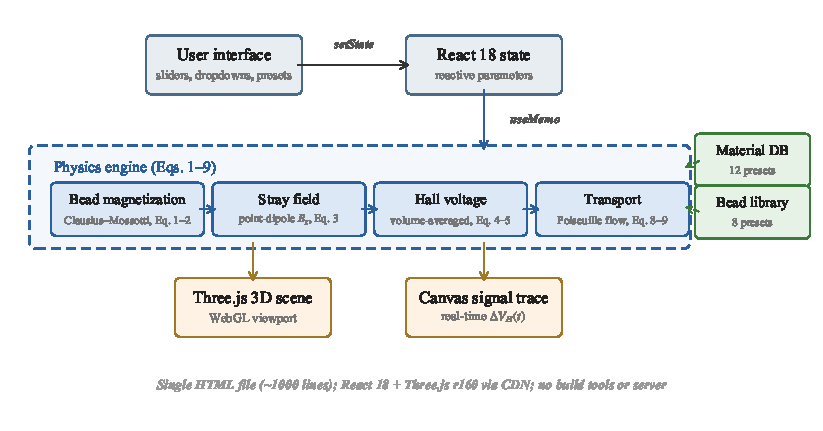
\includegraphics[width=\linewidth]{figures/fig1_architecture.pdf}
\caption{Data-flow architecture of the open implementation. User interactions update
React state, which triggers memoized physics computations
(Equations~\eqref{eq:moment}--\eqref{eq:vh}). Results feed the Three.js 3D scene, the
HTML5 Canvas signal trace, and the 2D axisymmetric FEM solver. The simulation loop
uses adaptive sub-stepping to capture narrow signal peaks; parametric sweeps bypass
the animation loop and evaluate the equations directly.\label{fig:architecture}}
\end{figure}

The interface is organized into pages reached from a tabbed header: a landing page;
a Simulator with real-time bead animation, a live $\Delta V_H$ signal trace with
superimposed noise, and a batch mode with per-bead detection statistics; a Designer
for sensor material, geometry, and bead selection with computed physics properties;
an Analysis page hosting the parametric sweep engine with CSV export; a Theory page
presenting the governing equations and data tables; and a FEM Solver page.
Figure~\ref{fig:screenshot} shows the Simulator page at the Design~II configuration.
The volume-averaging quadrature (Equation~\eqref{eq:avgbz}) uses a
$16 \times 16 \times 8$ grid; a convergence study at Design~II parameters
(Section~\ref{sec:validation}) shows that this resolution is converged. The
parametric sweep engine evaluates $\Delta V_H$ across user-specified ranges of bead
diameter, sensor size, flow velocity, applied field, channel height, height above
the sensor, or gate voltage by computing the equations directly; in multi-material
mode it iterates over all 12 presets at each sweep point, producing overlaid curves.

\begin{figure}[H]
\centering
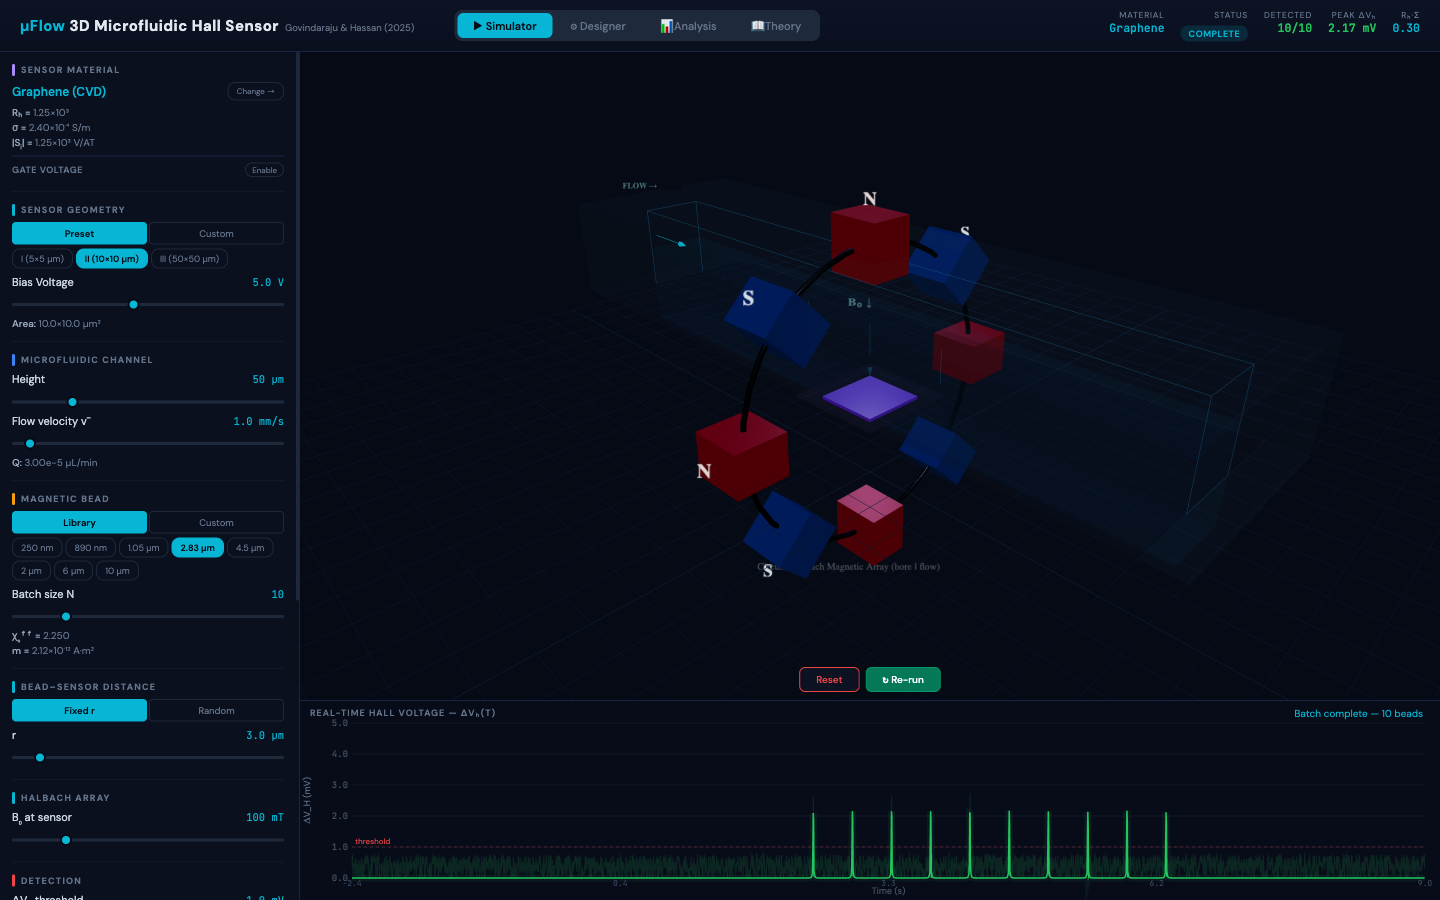
\includegraphics[width=\linewidth]{figures/fig2_screenshot.png}
\caption{Simulator page at the Design~II configuration
($w = \SI{10}{\micro\meter}$, $t = \SI{1}{\micro\meter}$, magnetite
\SI{6}{\micro\meter} bead, $B_0 = \SI{50}{\milli\tesla}$,
$V_{\text{bias}} = \SI{5}{\volt}$, $\bar{v} = \SI{1}{\milli\meter\per\second}$). The
left sidebar exposes material, geometry, channel, and detection controls; the center
viewport renders the PDMS channel, the Hall chip, the Halbach array, and a bead in
transit; the bottom panel plots the live $\Delta V_H$ trace with a noise-injected
overlay and detection threshold.\label{fig:screenshot}}
\end{figure}

% ---------------------------------------------------------------------
\subsubsection{In-App 2D Axisymmetric FEM Solver}
\label{sec:fem}

The implementation includes a 2D axisymmetric finite-element magnetostatic solver
that validates the point-dipole approximation without external software. The solver
computes the perturbation field $\Delta B_z$ from a magnetized bead using the
magnetic scalar potential formulation,
$\tfrac{1}{r}\partial_r(r\mu_r\partial_r\varphi) + \partial_z(\mu_r\partial_z\varphi)
= 0$, on a structured triangular mesh with adaptive refinement near the bead and
sensor, solved by a preconditioned conjugate-gradient method. Four mesh resolutions
are available, from coarse (${\sim}3200$ elements) to ultra (${\sim}39{,}200$
elements). The FEM page displays the $\Delta B_z$ field map, the mesh overlay, and a
side-by-side comparison of the FEM and analytical dipole profiles at the sensor
plane, with the height-to-radius ratio $h/r_b$ reported alongside the result. At
$h/r_b > 3$ the dipole approximation agrees with the FEM solution to within a few
percent; at $h/r_b \sim 1$ the deviation widens as finite bead-volume effects become
significant. The solver lets a user judge where the dipole approximation degrades for
any configuration without a commercial FEM license.

% =====================================================================
\section{Results}
\label{sec:results}
% =====================================================================

% ---------------------------------------------------------------------
\subsection{Validation Against FEM-BEM}
\label{sec:validation}

We validate the analytical model against the three sensor designs characterized in
our companion COMSOL FEM-BEM study \cite{govindaraju2025}.
Table~\ref{tab:designs} lists the design parameters and Table~\ref{tab:validation}
presents the validation results, also shown graphically in
Figure~\ref{fig:validation}.

\begin{table}[H]
\caption{Sensor design configurations from Reference~\cite{govindaraju2025}. All use
$R_H = \SI{1.25e-3}{\meter\cubed\per\coulomb}$,
$\sigma = \SI{1040}{\siemens\per\meter}$, $V_{\text{bias}} = \SI{5}{\volt}$,
$B_0 = \SI{50}{\milli\tesla}$, magnetite beads ($\mu_r = 10$). The area ratio is
$\pi r_b^2 / (w l)$ for a square sensor ($l = w$).\label{tab:designs}}
\begin{tabularx}{\textwidth}{Xccc}
\toprule
\textbf{Parameter} & \textbf{Design I} & \textbf{Design II} & \textbf{Design III} \\
\midrule
Sensor width $w$ ($\mu$m)         & 5    & 10   & 50 \\
Sensor thickness $t$ ($\mu$m)     & 0.5  & 1    & 1 \\
Bead diameter $d_b$ ($\mu$m)      & 2    & 6    & 10 \\
Bead-center height $r$ ($\mu$m)   & 1    & 3    & 5 \\
Bead-to-sensor area ratio         & 0.13 & 0.28 & 0.03 \\
\bottomrule
\end{tabularx}
\end{table}

\begin{table}[H]
\caption{Validation of the analytical model against COMSOL FEM-BEM results
\cite{govindaraju2025}, bead positioned directly above the sensor center.
\label{tab:validation}}
\begin{tabularx}{\textwidth}{Xccccc}
\toprule
\textbf{Design} & \textbf{COMSOL (mV)} & \textbf{Model (mV)} &
\textbf{Deviation (\%)} & \textbf{Sign} & \textbf{Area Ratio} \\
\midrule
I ($5\times5$\,$\mu$m)   & 21.375 & 16.63 & 22.2 & below & 0.13 \\
II ($10\times10$\,$\mu$m) & 42.79  & 44.86 & 4.8  & above & 0.28 \\
III ($50\times50$\,$\mu$m) & 3.056  & 2.58  & 15.6 & below & 0.03 \\
\bottomrule
\end{tabularx}
\end{table}

The analytical model reproduces the COMSOL Hall voltage to within 4.8\% at the
favorable bead-to-sensor area ratio of Design~II. At the off-optimum Designs~I and
III the point-dipole approximation deviates by 22\% and 16\%, consistent with its
known near-field limit at $h/r_b = 1$, where $r_b$ is the bead radius, the regime in
which the multipole expansion underlying the dipole form loses accuracy
\cite{griffiths}. All three designs operate at
$h/r_b = 1$, so the design-to-design spread is not an $h/r_b$ effect alone but a function
of the bead-to-sensor area ratio. Design~II's area ratio of 0.28 concentrates the
bead's stray-field footprint within the sensor active area, where the dipole
approximation captures most of the volume-averaged field. Design~I (area ratio 0.13)
under-covers the bead's near field with a small sensor, so the dipole under-estimates
the actual field by missing the finite-volume contribution. Design~III (area ratio
0.03) over-averages the bead's field across a large sensor, so the residual near-field
error has a larger fractional impact on the small mean. This pattern is the
expected behavior of the multipole expansion near the bead surface \cite{griffiths}
and motivates the in-app FEM solver (Section~\ref{sec:fem}) for users working at
$h/r_b \le 1.5$, where the dipole approximation degrades.

\begin{figure}[H]
\centering
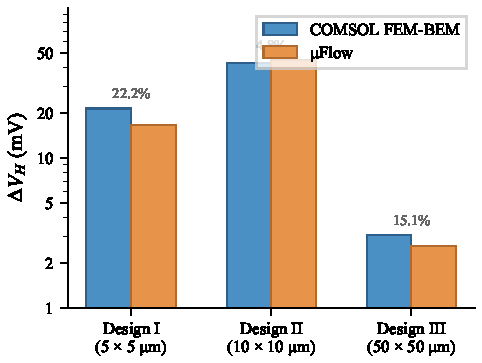
\includegraphics[width=\linewidth]{figures/fig3_validation.pdf}
\caption{Hall voltage predicted by the analytical model versus COMSOL FEM-BEM
\cite{govindaraju2025} for the three sensor designs. The model matches COMSOL to
within 4.8\% at the favorable area ratio of Design~II (0.28); at the off-optimum
Designs~I (area ratio 0.13) and III (area ratio 0.03) the point-dipole approximation
deviates by 22\% and 16\%, consistent with its near-field limit at $h/r_b = 1$.
\label{fig:validation}}
\end{figure}

The volume-averaging quadrature is converged at the resolution used. At Design~II
parameters, the $16 \times 16 \times 8$ grid gives $\Delta V_H = \SI{44.86}{\milli\volt}$,
within 0.044\% of a $64 \times 64 \times 32$ reference; the coarser
$8 \times 8 \times 4$ grid deviates by 0.18\% and the finer $32 \times 32 \times 16$
by 0.009\%. The quadrature error is therefore negligible compared with the
point-dipole near-field error. The in-app FEM solver provides an independent check:
at $h/r_b > 3$ the FEM and analytical results agree within 2\%, while at $h/r_b = 1$ the
deviation widens to \SIrange{5}{8}{\percent}, confirming that the built-in solver
captures the near-field effects the dipole approximation neglects.

% ---------------------------------------------------------------------
\subsection{Comparison with Published Detection Experiments}
\label{sec:expvalidation}

To assess the complete signal chain beyond the COMSOL comparison, we check the model
against published microfluidic Hall-effect bead-detection experiments. Exact
quantitative reproduction is limited because the published reports do not always
specify the precise bead-sensor distance, bias conditions, and sensor geometry needed
to reconstruct the measurement; we therefore assess consistency at the order-of-magnitude
level.

Mihajlovi\'{c} et al.\ detected a single commercial \SI{1.2}{\micro\meter} bead with
an InAs quantum-well micro-Hall sensor at \SI{40}{\micro\ampere} bias, reporting a
\SI{105}{\nano\volt} noise floor, a minimum detectable stray-field change of
${\sim}\SI{4.3}{\micro\tesla}$, and a bead signal at a signal-to-noise ratio of a few
\cite{mihajlovic2005}. The bead signal is therefore on the order of hundreds of
nanovolts. The model's InAs/AlSb 2DEG preset
($S_I = \SI{625}{\volt\per\ampere\per\tesla}$) predicts $\Delta V_H \approx
\SI{1}{\micro\volt}$ for a comparable bead and geometry, and the characteristic
bipolar waveform arises from the sign change in $B_z$ at lateral offsets
(Equation~\eqref{eq:dipole}). The predicted signal magnitude agrees with the
experimental scale to within an order of magnitude.

Besse et al.\ detected a single M-280 bead with a $2.4 \times 2.4$\,$\mu$m Si CMOS
Hall sensor ($S_I = \SI{175}{\volt\per\ampere\per\tesla}$, $R = \SI{8.5}{\kilo\ohm}$)
at $I_b = \SI{0.3}{\milli\ampere}$, with the bead at $r = \SI{7}{\micro\meter}$ and
the sensor thermal-noise-limited magnetic field resolution at
${\sim}\SI{0.2}{\micro\tesla\per\sqrt\hertz}$; they measured magnetic induction
variations exceeding \SI{20}{\micro\tesla} \cite{besse2002}. The corresponding
measured Hall voltage, $S_I I_b \Delta B \approx \SI{1}{\micro\volt}$ for the
\SI{20}{\micro\tesla} induction change, is in the microvolt range. The model
reproduces the order of the bead stray-field magnitude
(${\sim}10$--$\SI{100}{\micro\tesla}$ for an M-280 at micron distances) but its
signal-chain output for the Si CMOS preset is sensitive to the bias and film-thickness
values, which the report underspecifies; we therefore claim agreement only at the
order-of-magnitude level for the magnetic induction.

We do not include the Gabureac et al.\ nanocomposite sensor in the quantitative
comparison set. For their \SI{1}{\micro\meter}-bead configuration the model predicts
${\sim}\SI{44}{\micro\volt}$, while Gabureac et al.\ reported
\SIrange{100}{500}{\nano\volt}, a difference of about two orders of magnitude; their
\SI{500}{\nano\meter} nanocomposite sensor parameters are underspecified for this
model and fall outside its validated regime ($d_b/w = 2$, with the stray field
extending well beyond the sensor boundaries).

Mihajlovi\'{c} et al.\ separately identified, from $1/f$-limited noise analysis of
InAs micro-Hall sensors, a noise-optimal regime in which the sensor active area is
comparable to the bead footprint \cite{mihajlovic2007}. This geometry-matching
criterion is consistent with the
area-ratio optimum of 0.1--0.5 identified by the parametric sweeps
(Section~\ref{sec:geometry}) and with the observation by Kim et al.\ that the planar
Hall signal decreased once the sensor area exceeded the bead's stray-field footprint
\cite{kim2014}.

% ---------------------------------------------------------------------
\subsection{Cross-Material Comparison}
\label{sec:crossmaterial}

Figure~\ref{fig:materials} compares the Hall voltage produced by all 12 material
presets under identical Design~II geometry and bead conditions (\SI{6}{\micro\meter}
magnetite bead, $r = \SI{3}{\micro\meter}$, $B_0 = \SI{50}{\milli\tesla}$,
$V_{\text{bias}} = \SI{5}{\volt}$).

\begin{figure}[H]
\centering
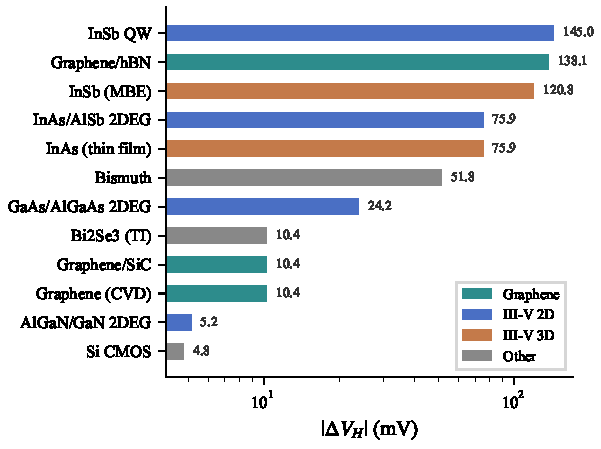
\includegraphics[width=\linewidth]{figures/fig5_materials.pdf}
\caption{Cross-material comparison of $\Delta V_H$ under identical geometry and bead
conditions (Design~II, $B_0 = \SI{50}{\milli\tesla}$, $V_{\text{bias}} = \SI{5}{\volt}$),
bars color-coded by material family. The signal tracks carrier mobility: InSb quantum
wells and graphene/hBN produce the strongest signals, while Si CMOS and AlGaN/GaN are
among the weakest.\label{fig:materials}}
\end{figure}

Because $\Delta V_H \propto R_H \sigma \propto \mu$ for a given geometry
(Equation~\eqref{eq:vh}), the mobility ratio between two materials predicts their
signal ratio under identical conditions, and the signals track carrier mobility. InSb
quantum wells ($\mu = \SI{42000}{\centi\meter\squared\per\volt\per\second}$) and
graphene/hBN ($\mu = \SI{40000}{\centi\meter\squared\per\volt\per\second}$) produce
the strongest intrinsic signals, while Si CMOS
($\mu = \SI{1400}{\centi\meter\squared\per\volt\per\second}$) and AlGaN/GaN
($\mu = \SI{1500}{\centi\meter\squared\per\volt\per\second}$) are among the weakest.
This ranking alone is insufficient for sensor selection because it ignores the
material-specific noise floor. Table~\ref{tab:noise} reports the noise-aware metrics
for a representative subset at Design~II geometry ($w = \SI{10}{\micro\meter}$,
$I_\text{bias} = \SI{10}{\micro\ampere}$, $\Delta f = f_\text{op} = \SI{1}{\kilo\hertz}$,
$T = \SI{300}{\kelvin}$). At these conditions graphene/hBN
($\Delta V_H = \SI{0.39}{\milli\volt}$, $\alpha_H = 10^{-5}$) produces about
$4.5\times$ the signal of Si CMOS ($\Delta V_H = \SI{0.086}{\milli\volt}$,
$\alpha_H = 5\times10^{-3}$), and its higher SNR is reinforced by the lower Hooge
parameter; the full 12-material set spans a wider range. Because
$V_{1/f} \propto \sqrt{\alpha_H / N}$ with $N = n_\text{tot} A$, a platform with low
carrier density (high $S_I$) can suffer higher $1/f$ noise from a reduced carrier
count, so the SNR ranking does not always follow the $\Delta V_H$ ranking. The
parametric sweep engine quantifies this trade-off for any user-specified $\alpha_H$.

\begin{table}[H]
\caption{Noise-aware metrics at Design~II geometry
($w = \SI{10}{\micro\meter}$, $I_\text{bias} = \SI{10}{\micro\ampere}$,
$\Delta f = f_\text{op} = \SI{1}{\kilo\hertz}$, $T = \SI{300}{\kelvin}$).
$V_n = \sqrt{V_\text{th}^2 + V_{1/f}^2}$;
$B_\text{min}$ is the minimum detectable field per $\sqrt{\hertz}$.\label{tab:noise}}
\begin{tabularx}{\textwidth}{Xcccccc}
\toprule
\textbf{Material} & \boldmath$\alpha_H$ &
\textbf{\boldmath$\Delta V_H$ (mV)} & \textbf{\boldmath$V_n$ (nV)} &
\textbf{SNR} & \textbf{\boldmath$B_\text{min}$ (nT/$\sqrt{\hertz}$)} \\
\midrule
Graphene/hBN  & $1\times10^{-5}$   & 0.39  & 190   & 2060 & 106 \\
InSb QW       & $5\times10^{-4}$   & 0.086 & 105   & 820  & 266 \\
CVD graphene  & $1.8\times10^{-4}$ & 0.086 & 709   & 122  & 1793 \\
InAs/AlSb     & $3.7\times10^{-3}$ & 0.043 & 159   & 271  & 806 \\
Si CMOS       & $5\times10^{-3}$   & 0.086 & 7440  & 12   & 18{,}800 \\
\bottomrule
\end{tabularx}
\end{table}

CVD graphene on SiO$_2$ ($\mu = \SI{3000}{\centi\meter\squared\per\volt\per\second}$)
offers a practical intermediate: its signal is well above Si CMOS while CVD growth is
compatible with wafer-scale integration \cite{shah2023}. AlGaN/GaN produces signals
comparable to Si CMOS but operates reliably above \SI{500}{\kelvin}
\cite{zhang2021}, and graphene/SiC is stable to \SI{770}{\kelvin} \cite{ciuk2019},
so both remain viable where graphene and InSb would degrade.

% ---------------------------------------------------------------------
\subsection{Geometry and Sensitivity Map}
\label{sec:geometry}

Figure~\ref{fig:distance} shows $\Delta V_H$ versus bead-sensor distance $r$ for the
three sensor sizes, computed by sweeping $r$ from \SIrange{0.5}{20}{\micro\meter}.
The characteristic $1/r^3$ dipolar decay is evident for all designs. At close range
($r < \SI{2}{\micro\meter}$) the \SI{5}{\micro\meter} sensor produces the strongest
signal because its small area concentrates the volume-averaged field; at larger
distances ($r > \SI{5}{\micro\meter}$) the \SI{10}{\micro\meter} sensor with a
\SI{6}{\micro\meter} bead dominates because the bead's larger dipole moment
($m \propto r_b^3$) compensates for the geometric dilution. Smaller sensors produce
stronger per-bead signals but are more sensitive to lateral misalignment, an effect
Tu et al.\ characterized experimentally \cite{tu2009}; larger sensors tolerate bead
position uncertainty but suffer geometric dilution.

\begin{figure}[H]
\centering
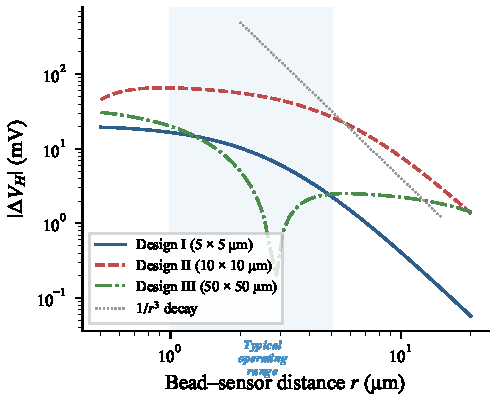
\includegraphics[width=\linewidth]{figures/fig4_distance.pdf}
\caption{Hall voltage $\Delta V_H$ versus bead-sensor distance for the three validated
sensor designs. The $1/r^3$ dipolar decay is evident on the log-log scale. Design~II
provides the strongest signal within the typical microfluidic operating range
($r = \SIrange{1}{5}{\micro\meter}$) due to its favorable bead-to-sensor area ratio.
\label{fig:distance}}
\end{figure}

Figure~\ref{fig:sensitivity} charts $\Delta V_H$ across the bead-diameter and
sensor-width plane, computed by the parametric sweep engine. The maximum lies along a
diagonal corresponding to bead-to-sensor area ratios between 0.1 and 0.5. The physical
origin is a competition between two scaling laws: the bead moment grows as
$m \propto d_b^3$ (Equation~\eqref{eq:moment}), favoring large beads, while the
volume-averaged stray field decreases as the sensor area grows beyond the bead's field
footprint, favoring small sensors. The optimum occurs where the bead's stray-field
extent approximately matches the sensor active area. For Dynabeads M-280
($d_b = \SI{2.8}{\micro\meter}$) the map predicts an optimal sensor width of
\SIrange{5}{15}{\micro\meter}; for M-450 ($d_b = \SI{4.5}{\micro\meter}$) the optimum
shifts to \SIrange{8}{25}{\micro\meter}. These values coincide with the regime,
identified by Mihajlovi\'{c} et al.\ as noise-optimal, in which the sensor active
area is comparable to the bead footprint
\cite{mihajlovic2007}, and with the sensor dimensions used in published single-bead
experiments \cite{mihajlovic2005,shah2023}.

\begin{figure}[H]
\centering
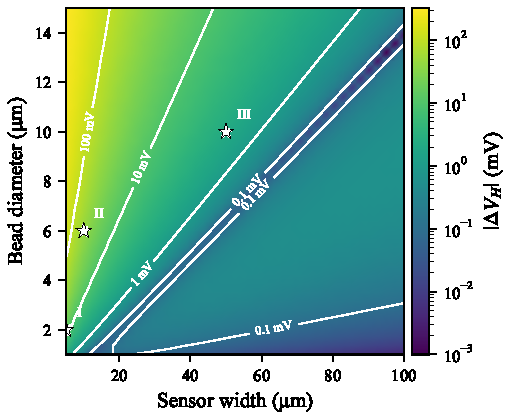
\includegraphics[width=\linewidth]{figures/fig7_sensitivity.pdf}
\caption{Sensitivity map: $\Delta V_H$ as a function of bead diameter and sensor width
($B_0 = \SI{50}{\milli\tesla}$, $V_{\text{bias}} = \SI{5}{\volt}$, bead centered at
$r = d_b/2 + \SI{0.1}{\micro\meter}$). The optimum lies along a diagonal corresponding
to bead-to-sensor area ratios of 0.1--0.5. Stars mark the three validated designs.
\label{fig:sensitivity}}
\end{figure}

% ---------------------------------------------------------------------
\subsection{Flow-Velocity Sensitivity}
\label{sec:flowsensitivity}

The flow velocity $\bar{v}$ affects detection through two competing mechanisms:
higher velocity increases throughput but shortens the transit time over the sensor,
reducing the integration window. Figure~\ref{fig:flowrate} shows the detection rate
and mean peak $\Delta V_H$ versus $\bar{v}$ for a batch of 20 beads at Design~II
geometry in range mode.

\begin{figure}[H]
\centering
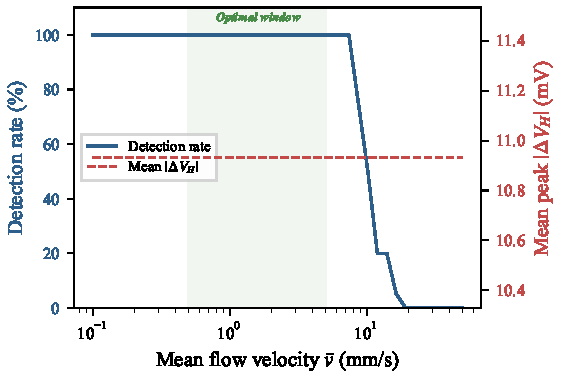
\includegraphics[width=\linewidth]{figures/fig6_flowrate.pdf}
\caption{Detection rate (left axis) and mean peak $\Delta V_H$ (right axis) versus
mean flow velocity for 20 beads at Design~II geometry in range mode. A detection window
emerges at $\bar{v} = \SIrange{0.5}{5}{\milli\meter\per\second}$, balancing throughput
against the requirement for adequate signal sampling.\label{fig:flowrate}}
\end{figure}

At low velocities ($\bar{v} < \SI{0.5}{\milli\meter\per\second}$) each bead spends many
seconds in the sensing zone, producing well-resolved pulses at low throughput. At
moderate velocities ($\bar{v} = \SIrange{0.5}{5}{\milli\meter\per\second}$) the
detection rate stays at 100\% and the peak $\Delta V_H$ is governed by bead height
rather than velocity, because adaptive sub-stepping ensures adequate sampling of the
signal peak. At high velocities ($\bar{v} > \SI{10}{\milli\meter\per\second}$) the
transit time $\tau_\text{transit} \approx w/v$ drops below the readout sampling
interval and some beads pass without being captured at maximum $\langle B_z\rangle$.
This window is consistent with the slow-flow regime of Aledealat et al.\, who
imaged beads transiting the Hall cross at ${\sim}\SI{3}{\micro\meter\per\second}$
(\SI{1}{\micro\liter\per\minute}), giving seconds-scale transits that resolved the
bipolar Hall transient as each bead entered, covered, and left the cross
\cite{aledealat2009}.

% ---------------------------------------------------------------------
\subsection{Batch Detection Statistics}
\label{sec:batch}

Batch mode injects $N$ beads (1--50) and records per-bead peak $\Delta V_H$, bead
height, and detection status. Table~\ref{tab:batch} reports the output for Design~II
with 10 beads at fixed height ($h = \SI{3.1}{\micro\meter}$) and in range mode
($h$ uniformly distributed across the channel).

\begin{table}[H]
\caption{Batch detection statistics for Design~II ($w = \SI{10}{\micro\meter}$,
$d_b = \SI{6}{\micro\meter}$, $\bar{v} = \SI{1}{\milli\meter\per\second}$,
$N = 10$ beads).\label{tab:batch}}
\begin{tabularx}{\textwidth}{Xcc}
\toprule
\textbf{Statistic} & \textbf{Fixed Height} & \textbf{Range Mode} \\
\midrule
Mean peak $\Delta V_H$ (mV)      & 44.9 & 28.7 \\
Standard deviation (mV)          & 0.7  & 12.3 \\
Coefficient of variation (\%)    & 1.7  & 42.9 \\
Detection rate (\%)              & 100  & 90 \\
\bottomrule
\end{tabularx}
\end{table}

In fixed-height mode the low coefficient of variation (1.7\%) confirms that signal
variation arises solely from numerical discretization. In range mode the coefficient
of variation rises to 42.9\% because beads at different heights experience different
stray-field amplitudes, and the detection rate falls to 90\% because beads near the
channel ceiling produce $\Delta V_H$ below threshold. This height-dependent variation
is physically realistic: Aledealat et al.\ recorded bipolar Hall transients from
superparamagnetic beads (\SI{2.6}{\micro\meter}, Bangs Laboratories) transiting an
InAs micro-Hall cross, with transient amplitudes set by the bead's stray field and
its position relative to the sensor, consistent with the $1/r^3$ scaling of the
volume-averaged field \cite{aledealat2009}.

% =====================================================================
\section{Discussion}
\label{sec:discussion}
% =====================================================================

\subsection{Design Rules and the Area-Ratio Optimum}

The parametric analysis yields three design rules. First, the bead-to-sensor area
ratio should lie between 0.1 and 0.5 for maximum $\Delta V_H$
(Figure~\ref{fig:sensitivity}). For Dynabeads M-280 ($d_b = \SI{2.8}{\micro\meter}$)
this corresponds to sensor widths of \SIrange{5}{15}{\micro\meter}. This area-ratio
optimum, obtained here from the signal-chain model, coincides with the regime,
identified by Mihajlovi\'{c} et al.\ as noise-optimal, in which the sensor active
area is comparable to the bead footprint, derived independently from
$1/f$-limited noise analysis of InAs micro-Hall sensors \cite{mihajlovic2007}. The two
criteria reach the same geometry from opposite directions, the signal-chain model by
maximizing the volume-averaged stray field and the noise analysis by minimizing the
$1/f$-limited detection limit, which strengthens the recommendation that sensor width
be matched to bead diameter. Second, detection reliability is maintained at
$\bar{v} = \SIrange{0.5}{5}{\milli\meter\per\second}$ for sensors in the
\SIrange{5}{50}{\micro\meter} range. Third, material selection requires noise-aware
analysis: while $\Delta V_H \propto \mu$ ranks materials by intrinsic signal, the SNR
depends on the Hooge parameter $\alpha_H$ through Equation~\eqref{eq:snr}
(Table~\ref{tab:noise}), so a high-mobility platform with poor noise performance can
achieve a lower SNR than a lower-mobility platform with superior $\alpha_H$.

\subsection{Regime of Validity of the Dipole Model}

The validation in Section~\ref{sec:validation} sets quantitative bounds on the
point-dipole approximation. The point-dipole form is the leading term of a
multipole expansion and loses accuracy as the bead-sensor separation approaches
the bead radius \cite{griffiths}; the built-in FEM solver quantifies this
deviation for each geometry, agreeing with the dipole model to within a few
percent at $h/r_b > 3$ and diverging as $h/r_b \to 1$. The model agrees with
COMSOL to within 4.8\% at Design~II, where the area ratio of 0.28 concentrates the
bead's stray-field footprint within the active area, but deviates by 22\% and 16\% at
the off-optimum Designs~I and III, where a small sensor under-covers the near field or
a large sensor over-averages it. All three designs sit at $h/r_b = 1$, the limit of the
dipole model, so the predictions should be trusted at $h/r_b \gtrsim 1.5$ and within the
area-ratio optimum, and treated as approximate near contact. For near-contact
geometries ($r \to r_b$), relevant to magnetic capture or surface-bound assays, the
multipole corrections that only a full FEM solver provides are needed; the in-app 2D
axisymmetric solver supplies this check without a commercial license. The bead
magnetization model is similarly bounded to $B_0 \lesssim \SI{200}{\milli\tesla}$,
above which a Langevin ensemble model is required, and the transport model assumes
fully developed laminar flow valid for $\text{Re} < 1$ \cite{hewlin2023}. The model
treats each bead independently, which holds for the dilute suspensions typical of
immunoassays but breaks down where dipolar coupling forms bead chains.

\subsection{Comparison to FEM Cost}

The analytical substitution replaces the volumetric FEM-BEM solve with a closed-form
evaluation of Equations~\eqref{eq:moment}--\eqref{eq:vh}.
Table~\ref{tab:performance} reports indicative costs. A single $\Delta V_H$ evaluation
completes in under \SI{1}{\milli\second}; a 100-point geometry sweep that a companion
COMSOL study estimated at ${\sim}\SI{8}{\hour}$ \cite{govindaraju2025} finishes in
\SI{0.3}{\second}. The speedup is a property of the analytical approximation, not an
algorithmic improvement over FEM, and applies only in the regime where the model is
validated; outside it, the cost advantage is moot and the in-app FEM solver or an
external package is the appropriate tool.

\begin{table}[H]
\caption{Indicative computational cost on a 2023 MacBook Pro (M2, Chrome). COMSOL
estimates from Reference~\cite{govindaraju2025}.\label{tab:performance}}
\begin{tabularx}{\textwidth}{Xcc}
\toprule
\textbf{Task} & \textbf{Analytical Model} & \textbf{COMSOL (est.)} \\
\midrule
Single $\Delta V_H$ evaluation        & ${<}\SI{1}{\milli\second}$ & ${\sim}\SI{5}{\minute}$ \\
100-point geometry sweep              & \SI{0.3}{\second}          & ${\sim}\SI{8}{\hour}$ \\
$12 \times 100$ material-geometry sweep & \SI{3}{\second}          & ${\sim}4$ days \\
20-bead batch with statistics         & \SI{5}{\second}            & Not available \\
In-app FEM solve (fine mesh)          & \SI{2}{\second}            & N/A \\
\bottomrule
\end{tabularx}
\end{table}

% =====================================================================
\section{Conclusions}
\label{sec:conclusions}
% =====================================================================

We presented a coupled closed-form analytical model of the microfluidic Hall-effect
magnetic-bead detection signal chain, combining Clausius--Mossotti bead magnetization
with a volume-fraction correction, a point-dipole stray field, a volume-averaged Hall
voltage with geometric correction, Poiseuille transport, and a Johnson--Nyquist/Hooge
$1/f$ noise framework over a database of 12 sensor platforms. Benchmarked against a
companion COMSOL FEM-BEM study, the model reproduces the Hall voltage to within 4.8\%
at the favorable bead-to-sensor area ratio of Design~II; at the off-optimum Designs~I
and III the point-dipole approximation deviates by 22\% and 16\%, consistent with its
known near-field limit at $h/r_b = 1$. The model yields design rules: a bead-to-sensor
area-ratio optimum of 0.1--0.5 that coincides with the independent noise-optimal width
criterion of Mihajlovi\'{c} et al., a cross-material signal-to-noise ranking in which
signals track carrier mobility, and a flow-velocity detection window of
\SIrange{0.5}{5}{\milli\meter\per\second}. The predicted signal magnitudes are
consistent at the order-of-magnitude level with published InAs and Si CMOS detection
experiments. We release the model as an open, no-install browser implementation with
an in-app 2D axisymmetric magnetostatic FEM solver that quantifies where the dipole
approximation degrades; the application is deployed at \url{https://uflow.studio} and
its source is released under AGPL-3.0-or-later at
\url{https://github.com/hg293/microfluidic-hall-sensor}.

% =====================================================================
% BACK MATTER
% =====================================================================

\vspace{6pt}

\authorcontributions{Conceptualization, H.G.\ and U.H.; methodology, H.G.\ and U.H.;
software, H.G.; validation, H.G.; formal analysis, H.G.; investigation, H.G.; data
curation, H.G.; writing---original draft preparation, H.G.;
writing---review and editing, H.G.\ and U.H.; visualization, H.G.; supervision, U.H.;
project administration, U.H.; funding acquisition, U.H. All authors have read and
agreed to the published version of the manuscript.}

\funding{This work was supported by the National Science Foundation
%% TODO: insert NSF award number(s) before submission
and the Department of Electrical and Computer Engineering at Rutgers,
The State University of New Jersey.}

\institutionalreview{Not applicable.}

\informedconsent{Not applicable.}

\dataavailability{The source code, build script, license, and example assets are
openly available on GitHub at \url{https://github.com/hg293/microfluidic-hall-sensor}
under the GNU Affero General Public License v3.0 or later (AGPL-3.0-or-later), with
trademark, citation, and patent reservations in the repository \texttt{NOTICE.md}.
The running application is publicly accessible at \url{https://uflow.studio}. An
archived snapshot of the version described here is deposited at Zenodo
(DOI: %% TODO: insert Zenodo DOI once minted
). No
experimental datasets were generated for this study; the simulation outputs reported
in Section~\ref{sec:results} are reproducible from the deployed application and from
the value-computation script in the repository.}

\acknowledgments{The authors thank the Rutgers Department of Electrical and Computer
Engineering for computational resources and the maintainers of the COMSOL companion
study for the FEM-BEM benchmark data.}

\conflictsofinterest{The authors declare no conflict of interest. The funders had no
role in the design of the study; in the collection, analyses, or interpretation of
data; in the writing of the manuscript; or in the decision to publish the results.}

% --- Generative AI disclosure (MDPI policy) ---
\vspace{6pt}
\noindent\textbf{Use of Generative AI:} During the preparation of this manuscript the
authors used ChatGPT (OpenAI) and GitHub Copilot to assist with drafting and editing
the text. After using these tools the authors reviewed and edited the content and take
full responsibility for the content of the published article.

% =====================================================================
% REFERENCES
% =====================================================================
\begin{adjustwidth}{-\extralength}{0cm}
\reftitle{References}
\bibliography{references}
\end{adjustwidth}

\end{document}
